

\chapter{Turnstiles in Stellarator fields}

the biosavart and the interpolated field. all the gym00 configurations

\section{QUASR configurations}

\section{Configuration \#0229079}

\section{Configuration \#0928241}

\section{Configuration \#1329594}

\section{Wendelstein-7X}

\begin{figure}[h!]
    \centering
    \begin{subfigure}[c]{0.49\textwidth}
        \centering
        \includegraphics[width=\textwidth]{}
        \caption{}
        \label{fig:}
    \end{subfigure}
    \hfill
    \begin{subfigure}[c]{0.49\textwidth}
        \centering
        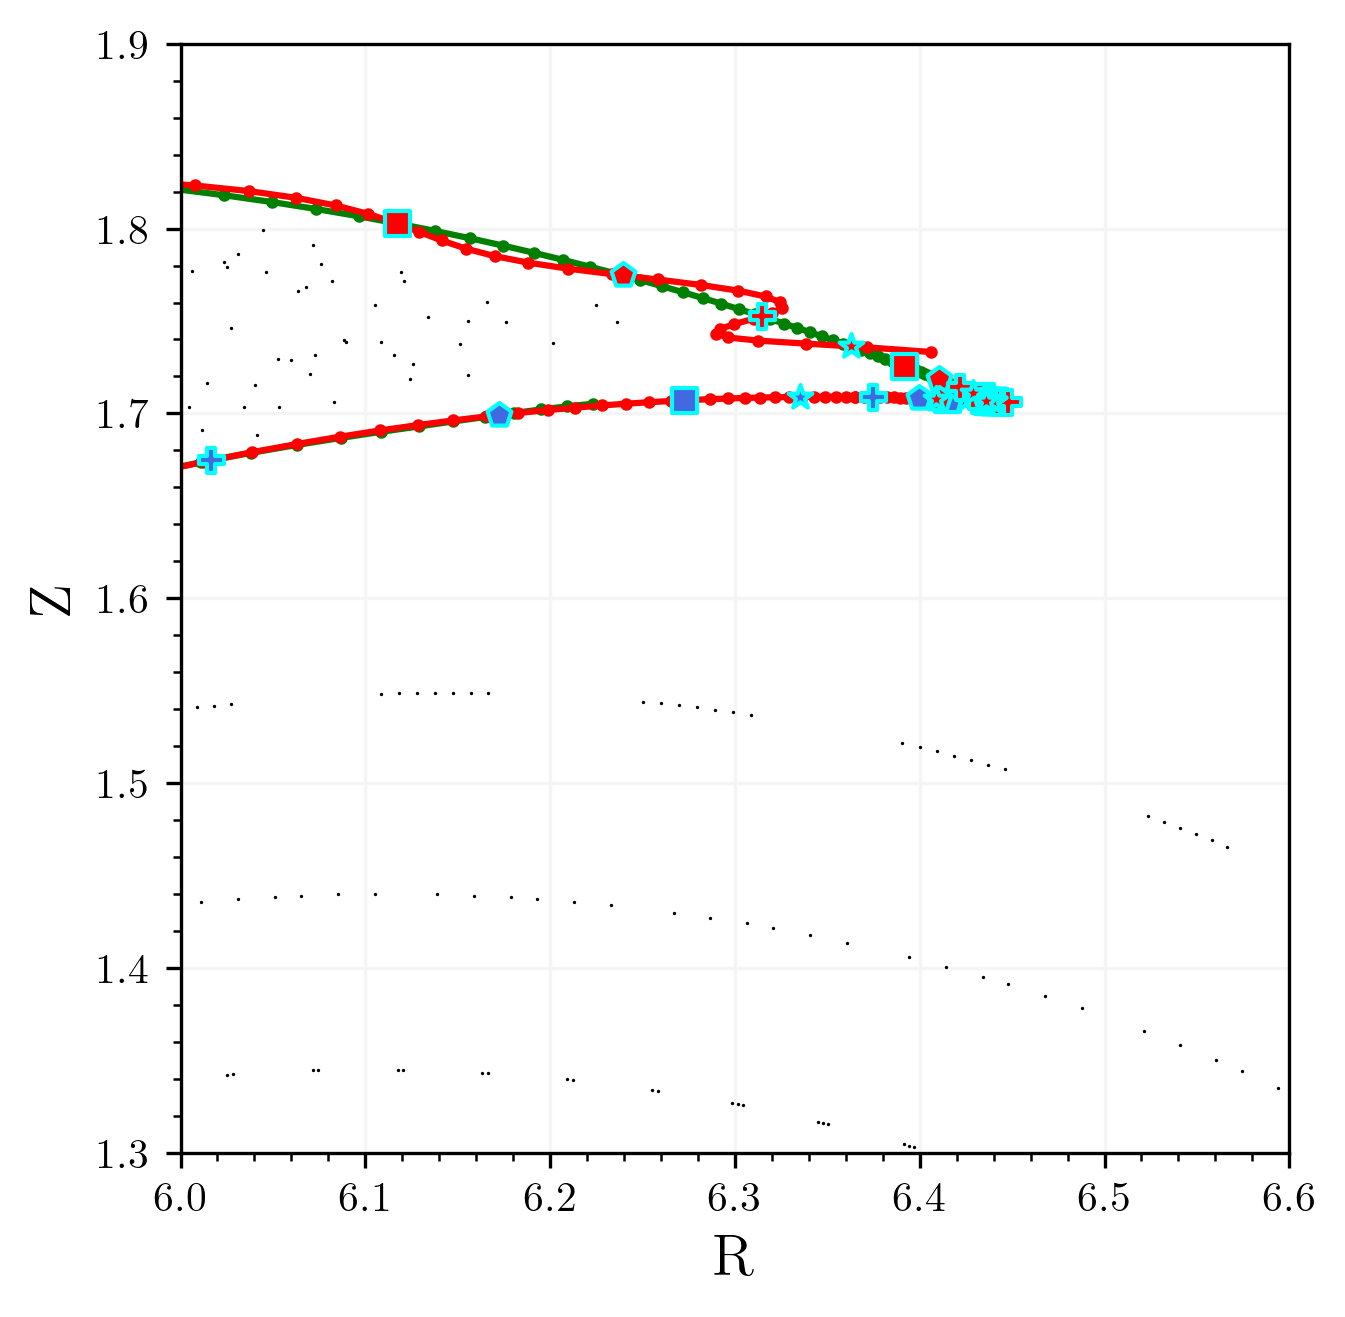
\includegraphics[width=\textwidth]{images/high-aspect-ratio/closeup.png}
        \caption{}
        \label{}
    \end{subfigure}
    \caption{}
    \label{}
\end{figure}

explanation of what it is, thanks to mat

\begin{figure}[H]
    \centering
    \begin{minipage}{0.45\textwidth} % Adjust width as needed
        \centering
        \begin{subfigure}[b]{\textwidth}
            \centering
            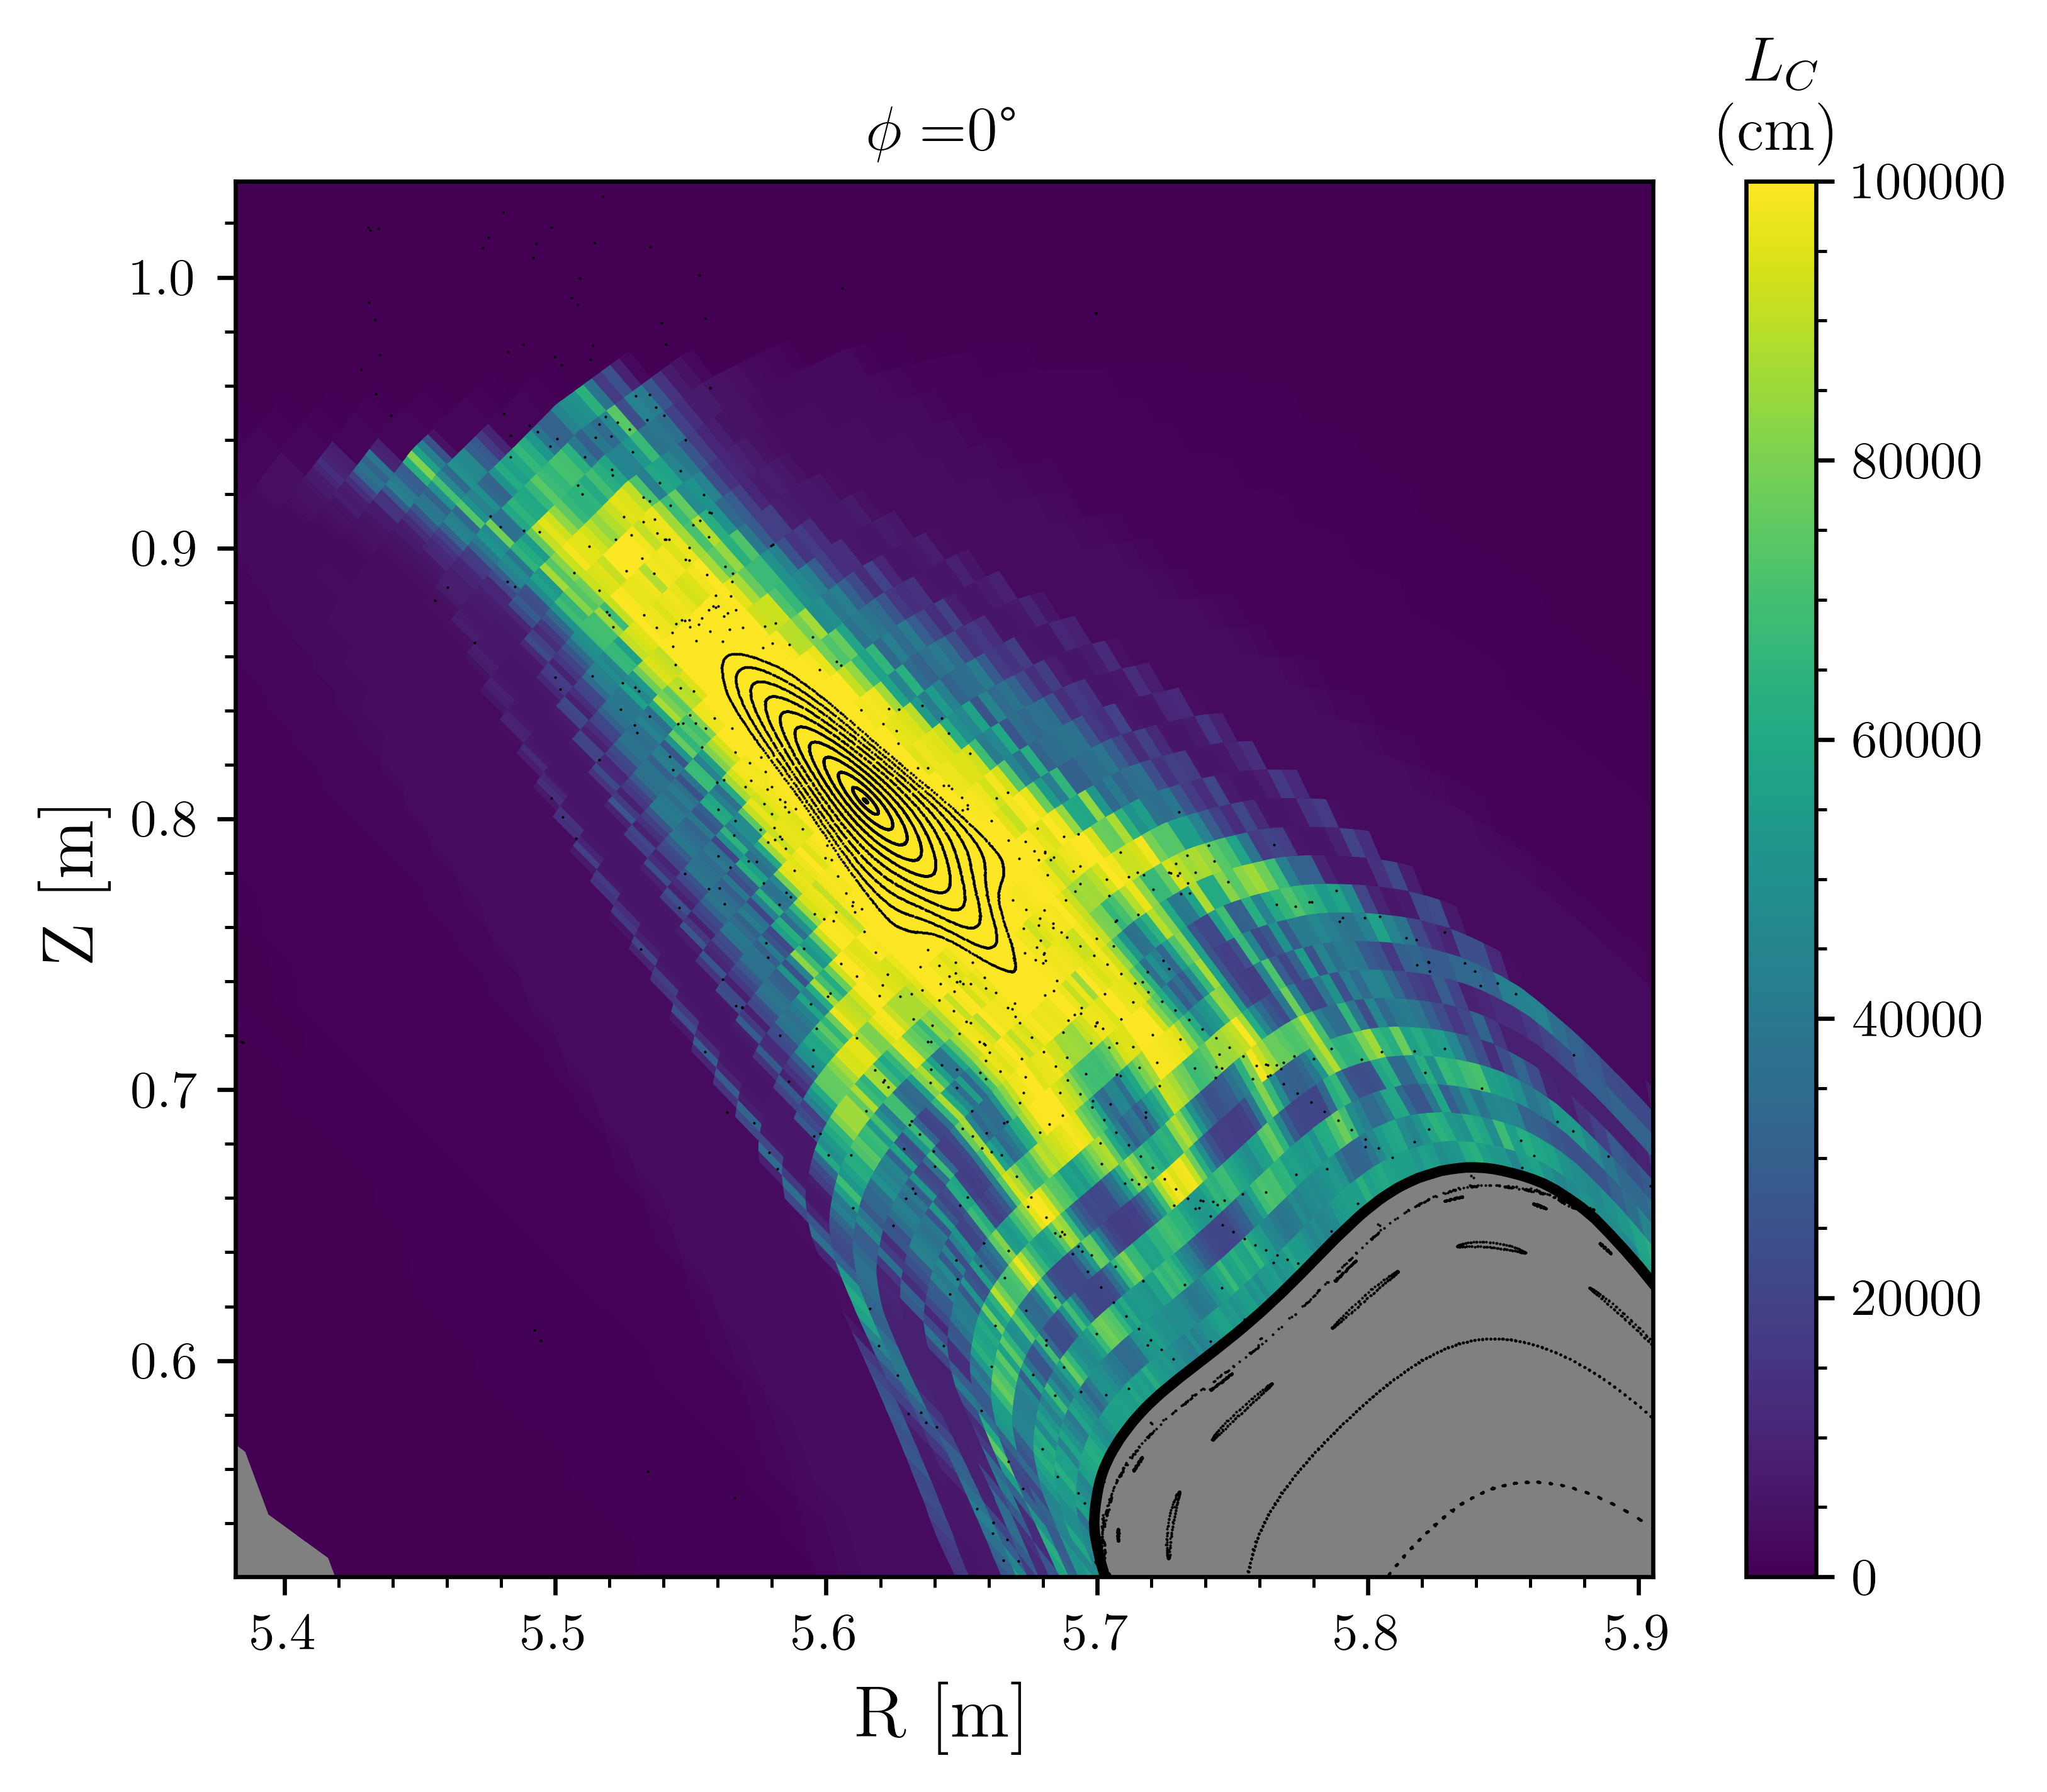
\includegraphics[width=\textwidth]{images/w7x-gym00-1750/gym00_1750_cnpoints.png}
            \caption{}
            \label{fig:}
        \end{subfigure}
        \vfill
        \vspace{10px}
        \vfill
        \begin{subfigure}[b]{0.99\textwidth}
            \centering
            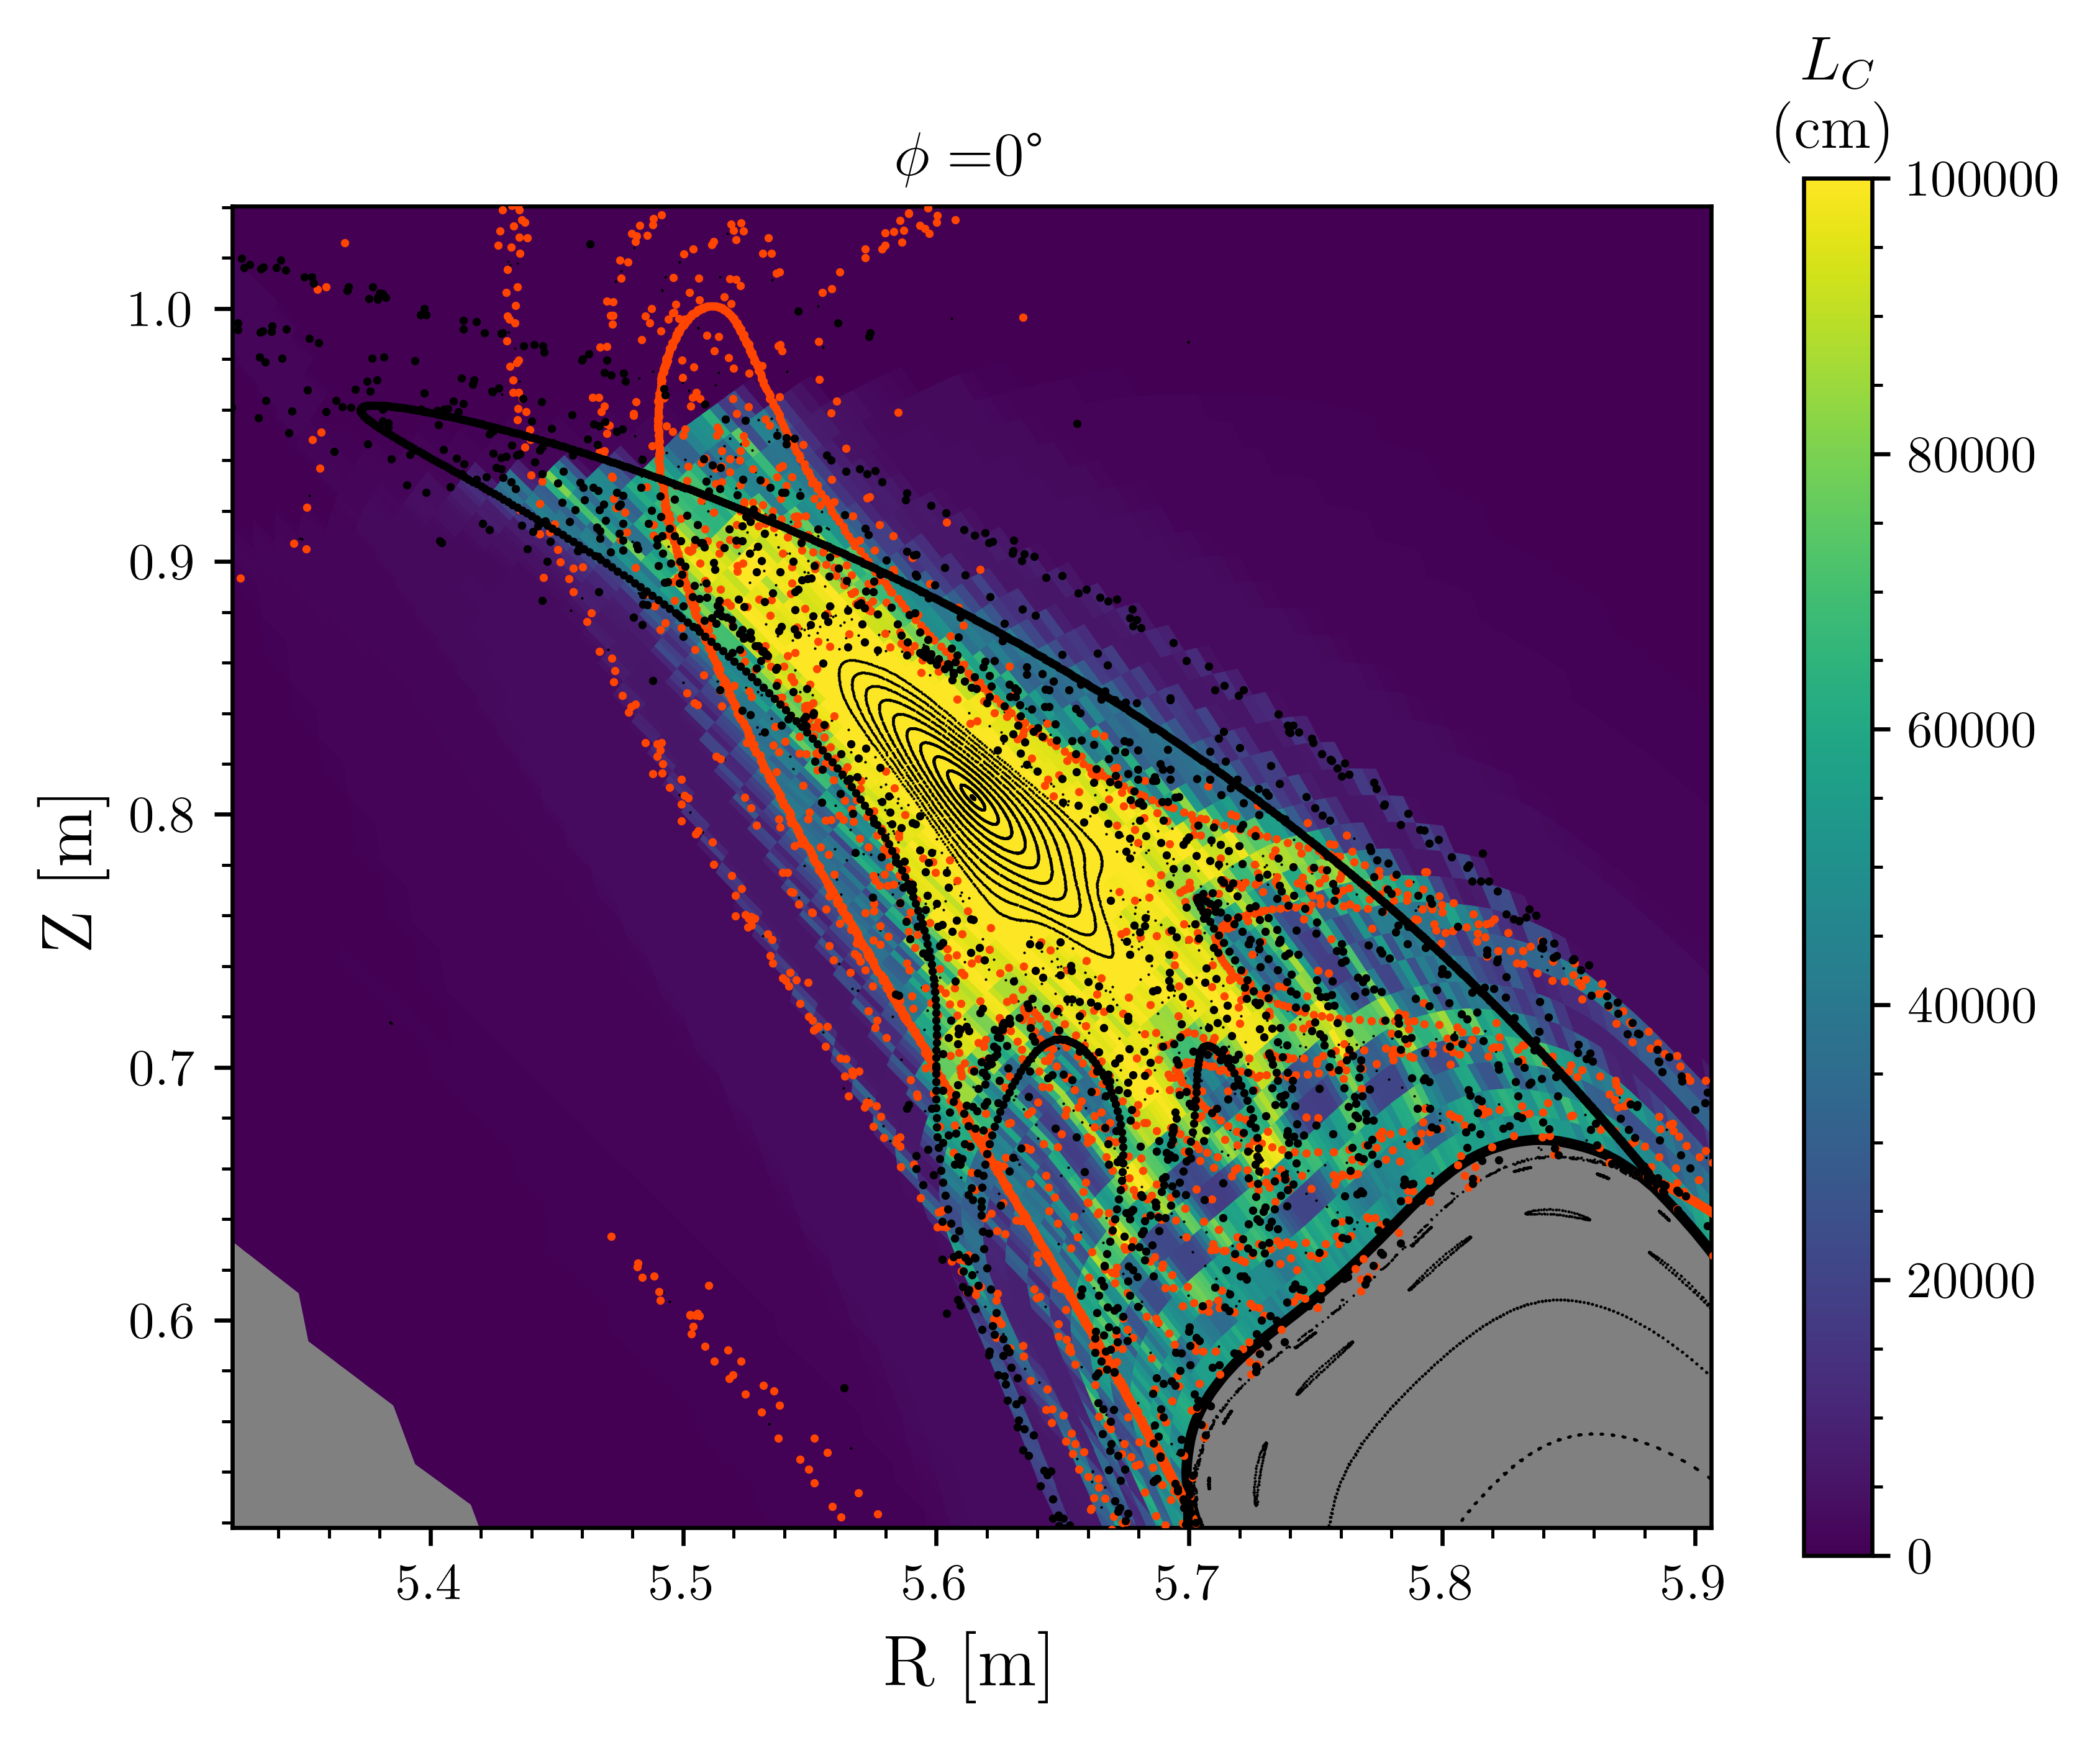
\includegraphics[width=\textwidth]{images/w7x-gym00-1750/gym00_1750_points.png}
            \caption{}
            \label{fig:}
        \end{subfigure}
    \end{minipage}%
    \begin{minipage}{0.5\textwidth} % Adjust width as needed
        \centering
        \begin{subfigure}[b]{\textwidth}
            \centering
            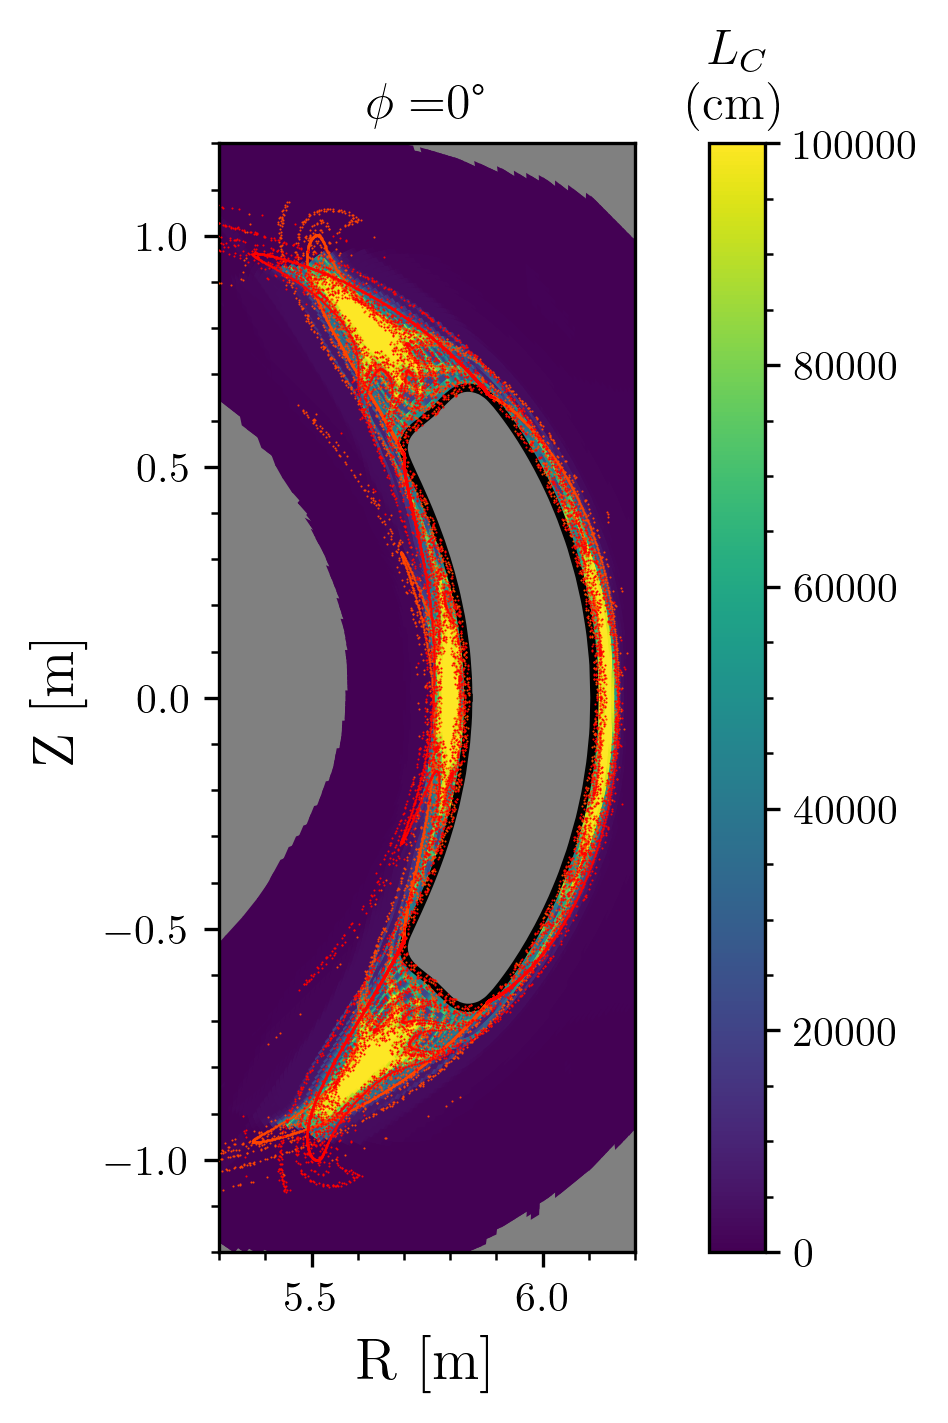
\includegraphics[width=\textwidth]{images/w7x-gym00-1750/gym00_1750_connlength.png}
            \caption{}
            \label{fig:}
        \end{subfigure}
    \end{minipage}
    \caption{}
    \label{fig:}
\end{figure}


\section{Inner vs outer turnstiles}

\begin{table}[]
    \centering
    \begin{tabular}{c|c}
         &  \\
         & 
    \end{tabular}
    \caption{Caption}
    \label{tab:my_label}
\end{table}